\documentclass[11pt]{charter}

% El títulos de la memoria, se usa en la carátula y se puede usar el cualquier lugar del documento con el comando \ttitle
\titulo{Desarrollo de sensor de corriente} 

% Nombre del posgrado, se usa en la carátula y se puede usar el cualquier lugar del documento con el comando \degreename
\posgrado{Carrera de Especialización en Sistemas Embebidos} 
%\posgrado{Carrera de Especialización en Internet de las Cosas} 
%\posgrado{Carrera de Especialización en Intelegencia Artificial}
%\posgrado{Maestría en Sistemas Embebidos} 
%\posgrado{Maestría en Internet de las cosas}

% Tu nombre, se puede usar el cualquier lugar del documento con el comando \authorname
\autor{Ing. Santiago Esteva} 

% El nombre del director y co-director, se puede usar el cualquier lugar del documento con el comando \supname y \cosupname y \pertesupname y \pertecosupname
\director{Esp. Ing. Bucafusco Franco}
\pertenenciaDirector{FIUBA} 
% FIXME:NO IMPLEMENTADO EL CODIRECTOR ni su pertenencia
\codirector{} % si queda vacio no se deberíá incluir 
\pertenenciaCoDirector{}

% Nombre del cliente, quien va a aprobar los resultados del proyecto, se puede usar con el comando \clientename y \empclientename
\cliente{Cristian Muzzio}
\empresaCliente{Hitec S.R.L.}

% Nombre y pertenencia de los jurados, se pueden usar el cualquier lugar del documento con el comando \jurunoname, \jurdosname y \jurtresname y \perteunoname, \pertedosname y \pertetresname.
\juradoUno{Nombre y Apellido (1)}
\pertenenciaJurUno{pertenencia (1)} 
\juradoDos{Nombre y Apellido (2)}
\pertenenciaJurDos{pertenencia (2)}
\juradoTres{Nombre y Apellido (3)}
\pertenenciaJurTres{pertenencia (3)}
 
\fechaINICIO{23 de Octubre de 2020}		%Fecha de inicio de la cursada de GdP \fechaInicioName
\fechaFINALPlanificacion{18 de Diciembre de 2020} 	%Fecha de final de cursada de GdP
\fechaFINALTrabajo{19 de Noviembre de 2021}		%Fecha de defensa pública del trabajo final


\begin{document}

\maketitle
\thispagestyle{empty}
\pagebreak


\thispagestyle{empty}
{\setlength{\parskip}{0pt}
\tableofcontents{}
}
\pagebreak


\section{Registros de cambios}
\label{sec:registro}


\begin{table}[ht]
\label{tab:registro}
\centering
\begin{tabularx}{\linewidth}{@{}|c|X|c|@{}}
\hline
\rowcolor[HTML]{C0C0C0} 
Revisión & \multicolumn{1}{c|}{\cellcolor[HTML]{C0C0C0}Detalles de los cambios realizados} & Fecha      \\ \hline
1.0      & Creación del documento                                          & 23/10/2020 \\ \hline
1.1      & Desarrollo hasta sección 6 inclusive                            & 05/11/2020 \\ \hline
1.2      & Correcciones e historias de usuario                            & 15/11/2020 \\ \hline
      &                                                   &  \\ \hline
\end{tabularx}
\end{table}

\pagebreak



\section{Acta de constitución del proyecto}
\label{sec:acta}

\begin{flushright}
Buenos Aires, \fechaInicioName
\end{flushright}

\vspace{2cm}

Por medio de la presente se acuerda con el Ing. \authorname\hspace{1px} que su Trabajo Final de la \degreename\hspace{1px} se titulará ``\ttitle'', consistirá esencialmente en el prototipo preliminar de un desarrollo de un sensor de corriente de tres fases capaz de medir, procesar e informar diversos parámetros necesarios para el mantenimiento predictivo en la industria, y tendrá un presupuesto preliminar estimado de 600 hs de trabajo y \textcolor{red}{\$XXX}, con fecha de inicio \fechaInicioName\hspace{1px} y fecha de presentación pública \fechaFinalName.

Se adjunta a esta acta la planificación inicial.

\vfill

% Esta parte se construye sola con la información que hayan cargado en el preámbulo del documento y no debe modificarla
\begin{table}[ht]
\centering
\begin{tabular}{ccc}
\begin{tabular}[c]{@{}c@{}}Ariel Lutenberg \\ Director posgrado FIUBA\end{tabular} & \hspace{2cm} & \begin{tabular}[c]{@{}c@{}}\clientename \\ \empclientename \end{tabular} \vspace{2.5cm} \\ 
\multicolumn{3}{c}{\begin{tabular}[c]{@{}c@{}} \supname \\ Director del Trabajo Final\end{tabular}} \vspace{2.5cm} \\
%\begin{tabular}[c]{@{}c@{}}\jurunoname \\ Jurado del Trabajo Final\end{tabular}     &  & \begin{tabular}[c]{@{}c@{}}\jurdosname\\ Jurado del Trabajo Final\end{tabular}  \vspace{2.5cm}  \\
%\multicolumn{3}{c}{\begin{tabular}[c]{@{}c@{}} \jurtresname\\ Jurado del Trabajo Final\end{tabular}} \vspace{.5cm}                                                                     
\end{tabular}
\end{table}




\section{Descripción técnica-conceptual del proyecto a realizar}
\label{sec:descripcion}

En la industria química existen procesos continuos de fabricación que deben ser controlados de forma permanente para asegurar una calidad constante entre lotes de un mismo producto. Sumado a los controles en tiempo de ejecución, existen técnicas de mantenimiento predictivo que permiten prever posibles fallas en los actuadores del proceso que implican paros de emergencia o tiempos muertos, que concluyen en pérdidas parciales o totales del lote.
Dado que en la mayoría de estos procesos se utilizan motores eléctricos como actuadores, se abre una gran posibilidad de desarrollar diversos tipos de sensores para aplicar mantenimiento predictivo. En la bibliografía se pueden encontrar diversos métodos relacionados a evaluar el desgaste de un motor mediante el análisis de su corriente de consumo. Es por ello que la empresa \empclientename necesita un sensor de corriente capaz de medir, procesar y comparar datos estadísticos en dominio del tiempo y frecuencia.

Actualmente la empresa presta un servicio de mantenimiento predictivo mediante la plataforma comercial \textit{teBox} de la firma Terative, con análisis y reportes de datos en la nube y se encuentra en la búsqueda de un sensor de corriente que se adecúe a su plataforma. El presente proyecto busca cubrir esta necesidad y propone desarrollar un sensor de corriente trifásico capaz de medir, procesar, almacenar y comunicar parámetros específicos a través de la plataforma \textit{teBox}.

En la figura \ref{fig:diagBloques} se presenta un diagrama en bloques del sensor que se propone desarrollar con el nombre comercial de teSensor-TC (\textit{Trifasic Current Sensor}) . Se observa la unidad central de procesamiento con sus periféricos, los circuitos necesarios para la adaptación de señales, alimentación y comunicación y los cuatro sensores externos.

\vspace{25px}

\begin{figure}[htpb]
\centering 
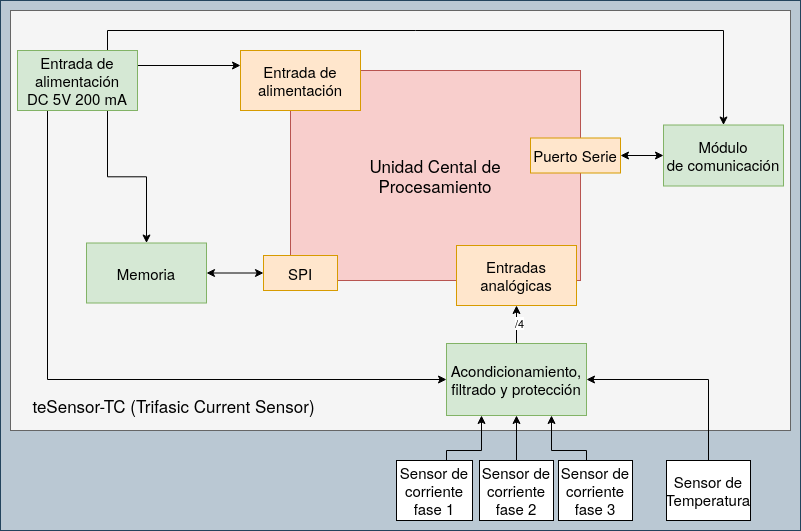
\includegraphics[width=.9\textwidth]{./Figuras/diagBloque.png}
\caption{Diagrama en bloques del sistema}
\label{fig:diagBloques}
\end{figure}

\vspace{25px}


El sensor debe medir los siguiente parámetros:
\begin{itemize}
\item Desplazamiento entre las tres fases
\item Valor estadístico (por fase) de corriente RMS AC 
\item Valor estadístico (por fase) de corriente DC
\item Valor estadístico (por fase) de factor de cresta
\item Valor pico de la corriente
\end{itemize}


Adicionalmente deberá procesar cada señal en frecuencia con la capacidad de extraer la frecuencia de máxima energía y energía de bandas predefinidas, contener una memoria externa para almacenar datos relacionados a valores de calibración de fábrica, valores de última calibración, máximos históricos de algunas variables de interés, fecha de cada dato almacenado, etc.

\section{Identificación y análisis de los interesados}
\label{sec:interesados}

\begin{table}[ht]
%\caption{Identificación de los interesados}
%\label{tab:interesados}
\begin{tabularx}{\linewidth}{@{}|l|X|X|l|@{}}
\hline
\rowcolor[HTML]{C0C0C0} 
Rol           & Nombre y Apellido & Organización 	& Puesto 	\\ \hline
Auspiciante y & \clientename      &\empclientename	&        	\\
Cliente		  &			   		  &					&        	\\ \hline
Responsable   & \authorname       & FIUBA        	& Alumno 	\\ \hline
Colaboradores & Martin Mello Teggia & FIUBA        	& Alumno 	\\ \hline
Orientador    & \supname	      & \pertesupname 	& Director	Trabajo final \\ \hline
Usuario final & Personal técnico del & \empclientename   	& Técnico       	\\ 
				& sector de instalaciones &              	&        	\\ \hline
\end{tabularx}
\end{table}
 
\begin{itemize}
\item Colaborador: Martín Mello Teggia, empleado de la empresa \empclientename  y estudiante de la especialización con gran experiencia en diseño de hardware y software.
\end{itemize}




\section{1. Propósito del proyecto}
\label{sec:proposito}

El propósito de este proyecto es desarrollar un sensor de corriente de tres fases capaz de medir, procesar e informar diversos parámetros necesarios para el mantenimiento predictivo en la industria química.

\section{2. Alcance del proyecto}
\label{sec:alcance}

El proyecto incluye los siguientes puntos:
\begin{itemize}
\item El diseño e implementación del hardware.
\item El desarrollo del firmware capaz de recolectar los datos, procesarlos y enviarlos mediante el protocolo de comunicación específico de \textit{teBox} en modelo maestro-esclavo.
\item Sensado de temperatura ambiental para conocer el modo de operación.
\item Desarrollo de una memoria técnica del proyecto.
\end{itemize}

El proyecto no incluye los siguientes puntos:
\begin{itemize}
\item El diseño y construcción de packaging asociado para la distribución del producto.
\item El análisis de los datos recolectados y procesados.
\end{itemize}

\section{3. Supuestos del proyecto}
\label{sec:supuestos}

Para el desarrollo del presente proyecto se supone que:

\begin{itemize}
\item Todos los materiales necesarios para la implementación serán suministrados por \empclientename.
\item La importación de componentes no estará restringida y tomará un tiempo menor a 3 meses.
\item Se contará con asistencia por parte de \empclientename \space para el montaje de los componentes en el PCB.
\item \empclientename \space cuenta con todos los equipos para la medición y validación del prototipo.
\end{itemize}


\section{4. Requerimientos de testing}
\label{sec:requerimientos}

A continuación se listan los requerimientos en prioridad descendente:

\begin{enumerate}
\item Grupo de requerimientos asociados al sistema
	\begin{enumerate}
	\item La alimentación por cable debe ser de 5 V con un consumo máximo de 200 mA. \label{req1}
	\item El sistema utilizará sensores disponibles comercialmente para la adquisición de la corriente y temperatura.
	\item El sistema deberá ser capaz de tomar muestras de los tres sensores de corriente en simultaneo al período de muestreo fijo.
	\item El sistema deberá poseer una memoria no volátil para registrar datos como valores máximos, parámetros de calibración, etc. 
	\item El sistema debe medir la temperatura ambiental de operación, rango de medición 0 - 50 centígrados.
	\item El sistema incorporará diseño y elementos que aseguren bajo consumo de energía (requerimiento \ref{req1}).
	\item Los indicadores de situación serán enviados mediante el protocolo de comunicación.
	\end{enumerate}
\item Grupo de requerimientos asociados a la comunicación de datos
	\begin{enumerate}
	\item El protocolo de comunicación está definido por la plataforma \textit{teBox}.
	\item El sensor se comporta como esclavo y la plataforma \textit{teBox} como maestro.
	\end{enumerate}
\item Grupo de requerimientos asociados con el sensor de corriente
	\begin{enumerate}
	\item El sensor debe ser de efecto Hall.
	\item El sensor debe detectar corriente continua, alterna y de pulsos.
	\item El sensor debe ser de núcleo partido.
	\item El sensor debe ser de bajo consumo (máximo 20 mA).
	\end{enumerate}
\end{enumerate}


\section{Historias de usuarios (\textit{Product backlog})}
\label{sec:backlog}

\begin{consigna}{red}
Descripción: En esta sección se deben incluir las historias de usuarios y su ponderación (\textit{history points}). Recordar que las historias de usuarios son descripciones cortas y simples de una característica contada desde la perspectiva de la persona que desea la nueva capacidad, generalmente un usuario o cliente del sistema. La ponderación es un número entero que representa el tamaño de la historia comparada con otras historias de similar tipo.
\end{consigna}

\section{5. Entregables principales del proyecto}
\label{sec:entregables}

\begin{itemize}
\item Prototipo funcional
\item Manual de uso
\item Diagrama esquemático electrónico del hardware
\item Código fuente
\item Manual de instalación
\item Informe final

\end{itemize}


\section{6. Desglose del trabajo en tareas}
\label{sec:wbs}

\begin{enumerate}
\item Análisis preliminar (48 hs)
	\begin{enumerate}
	\item Estudio sobre mantenimiento predictivo (10 hs)
	\item Investigación sobre posibles sensores de corriente (10 hs)
	\item Realizar el plan del proyecto (28 hs)
	\end{enumerate}
\item Hardware (140 hs)
	\begin{enumerate}
	\item Selección de componentes (12 hs)
	\item Diseño del circuito esquemático (28 hs)
	\item Diseño del PCB (30 hs)
	\item Fabricación y ensamblado del PCB (30 hs)
	\item Pruebas y validación del hardware (40 hs)
	\end{enumerate}
\item Firmware (154 hs)
	\begin{enumerate}
	\item Desarrollo de arquitectura del firmware  (16 hs)
	\item Diseño de firmware (32 hs)
	\item Análisis de riesgos de firmware (10 hs)
	\item Desarrollo de pruebas para firmware (32 hs)
	\item Programación del firmware (40 hs)
	\item Verificación y validación del firmware (24 hs)
	\end{enumerate}
\item Integración (157 hs)
	\begin{enumerate}
	\item Integración de los módulos constitutivos (32 hs)
	\item Pruebas de sensado (30 hs)
	\item Pruebas de almacenamiento de datos(30 hs)
	\item Pruebas de comunicación(30 hs)	
	\item Corrección de errores (35 hs)
	\end{enumerate}
\item Procesos finales (104 hs)
	\begin{enumerate}
	\item Elaboración del informe de avance (15 hs)
	\item Evaluación de requerimientos (25 hs)
	\item Elaboración de la memoria del proyecto (30 hs)
	\item Preparación de la presentación final (34 hs)
	\end{enumerate}
\end{enumerate}

Cantidad total de horas: 603 hs


\section{7. Diagrama de Activity On Node}
\label{sec:AoN}

\begin{consigna}{red}
Armar el AoN a partir del WBS definido en la etapa anterior. 

%La figura \ref{fig:AoN} fue elaborada con el paquete latex tikz y pueden consultar la siguiente referencia \textit{online}:

%\url{https://www.overleaf.com/learn/latex/LaTeX_Graphics_using_TikZ:_A_Tutorial_for_Beginners_(Part_3)\%E2\%80\%94Creating_Flowcharts}

\end{consigna}

\begin{figure}[htpb]
\centering 
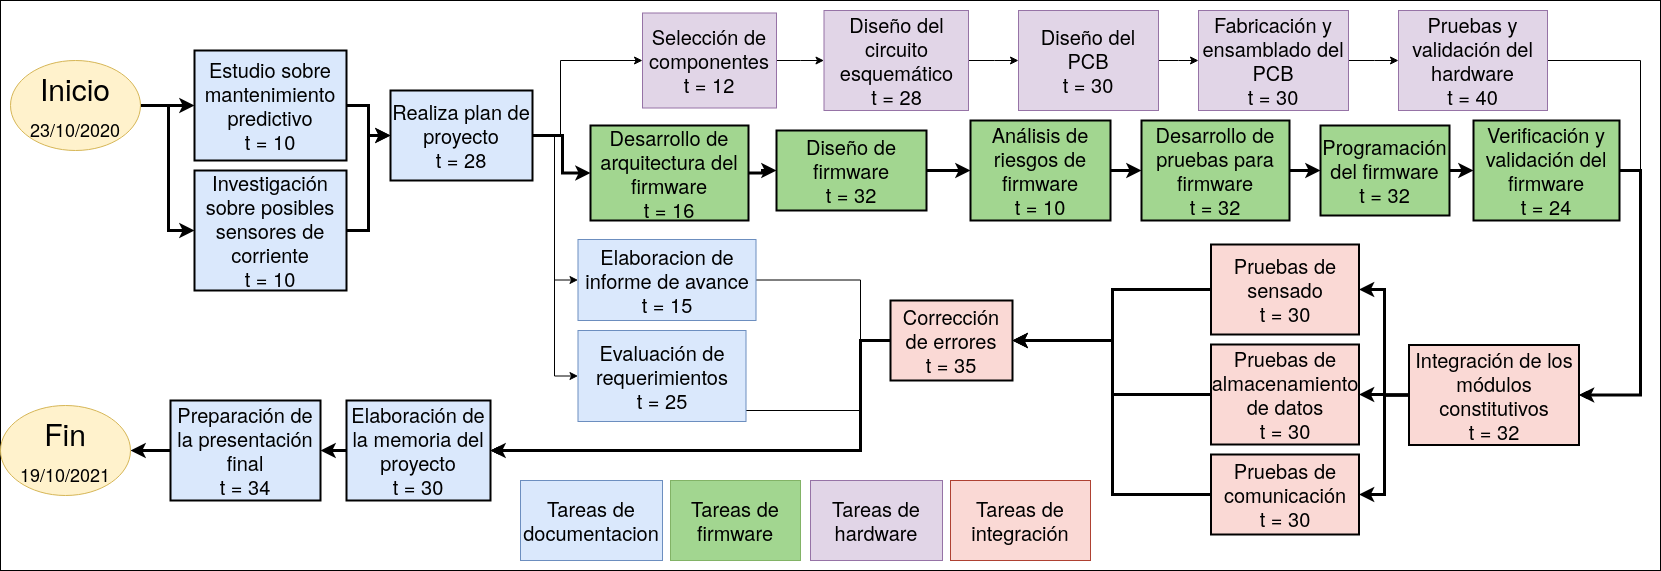
\includegraphics[width=.8\textwidth]{./Figuras/AoN.png}
\caption{Diagrama en \textit{Activity on Node}}
\label{fig:AoN}
\end{figure}

Indicar claramente en qué unidades están expresados los tiempos.
De ser necesario indicar los caminos semicríticos y analizar sus tiempos mediante un cuadro.
Es recomendable usar colores y un cuadro indicativo describiendo qué representa cada color, como se muestra en el siguiente ejemplo:



\section{8. Diagrama de Gantt}
\label{sec:gantt}

\begin{consigna}{red}
Utilizar el software Gantter for Google Drive o alguno similar para dibujar el diagrama de Gantt.

Existen muchos programas y recursos \textit{online} para hacer diagramas de gantt, entre las cuales destacamos:

\begin{itemize}
\item Planner
\item GanttProject
\item Trello + \textit{plugins}. En el siguiente link hay un tutorial oficial: \\ \url{https://blog.trello.com/es/diagrama-de-gantt-de-un-proyecto}
\item Creately, herramienta online colaborativa. \\\url{https://creately.com/diagram/example/ieb3p3ml/LaTeX}
\item Se puede hacer en latex con el paquete \textit{pgfgantt}\\ \url{http://ctan.dcc.uchile.cl/graphics/pgf/contrib/pgfgantt/pgfgantt.pdf}
\end{itemize}

Pegar acá una captura de pantalla del diagrama de Gantt, cuidando que la letra sea suficientemente grande como para ser legible. 
Si el diagrama queda demasiado ancho, se puede pegar primero la ``tabla'' del Gantt y luego pegar la parte del diagrama de barras del diagrama de Gantt.

Configurar el software para que en la parte de la tabla muestre los códigos del EDT (WBS).\\
Configurar el software para que al lado de cada barra muestre el nombre de cada tarea.\\
Revisar que la fecha de finalización coincida con lo indicado en el Acta Constitutiva.

En la figura \ref{fig:gantt}, se muestra un ejemplo de diagrama de gantt realizado con el paquete de \textit{pgfgantt}. En la plantilla pueden ver el código que lo genera y usarlo de base para construir el propio.

\begin{figure}[htbp]
\begin{center}
\begin{ganttchart}{1}{12}
  \gantttitle{2020}{12} \\
  \gantttitlelist{1,...,12}{1} \\
  \ganttgroup{Group 1}{1}{7} \\
  \ganttbar{Task 1}{1}{2} \\
  \ganttlinkedbar{Task 2}{3}{7} \ganttnewline
  \ganttmilestone{Milestone o hito}{7} \ganttnewline
  \ganttbar{Final Task}{8}{12}
  \ganttlink{elem2}{elem3}
  \ganttlink{elem3}{elem4}
\end{ganttchart}
\end{center}
\caption{Diagrama de gantt de ejemplo}
\label{fig:gantt}
\end{figure}

\end{consigna}

\section{9. Matriz de uso de recursos de materiales}
\label{sec:recursos}


\begin{table}
\label{tab:recursos}
\centering
\begin{tabularx}{\linewidth}{@{}|c|X|X|X|X|c|@{}}
\hline
\cellcolor[HTML]{C0C0C0} & \cellcolor[HTML]{C0C0C0} & \multicolumn{4}{c|}{\cellcolor[HTML]{C0C0C0}Recursos requeridos (horas)} \\ \cline{3-6} 
\multirow{-2}{*}{\cellcolor[HTML]{C0C0C0}\begin{tabular}[c]{@{}c@{}}Código\\ WBS\end{tabular}} & \multirow{-2}{*}{\cellcolor[HTML]{C0C0C0}\begin{tabular}[c]{@{}c@{}}Nombre \\ tarea\end{tabular}} & Material 1 & Material 2 & Material 3 & Material 4 \\ \hline
 &  &  &  &  &  \\ \hline
 &  &  &  &  &  \\ \hline
 &  &  &  &  &  \\ \hline
 &  &  &  &  &  \\ \hline
 &  &  &  &  &  \\ \hline
 &  &  &  &  &  \\ \hline
 &  &  &  &  &  \\ \hline
 &  &  &  &  &  \\ \hline 
 &  &  &  &  &  \\ \hline
 &  &  &  &  &  \\ \hline
 &  &  &  &  &  \\ \hline
 &  &  &  &  &  \\ \hline
 &  &  &  &  &  \\ \hline
 &  &  &  &  &  \\ \hline
 &  &  &  &  &  \\ \hline
 &  &  &  &  &  \\ \hline
 &  &  &  &  &  \\ \hline
 &  &  &  &  &  \\ \hline
 &  &  &  &  &  \\ \hline
 &  &  &  &  &  \\ \hline
 &  &  &  &  &  \\ \hline
 &  &  &  &  &  \\ \hline
 &  &  &  &  &  \\ \hline
 &  &  &  &  &  \\ \hline 
 &  &  &  &  &  \\ \hline
 &  &  &  &  &  \\ \hline
 &  &  &  &  &  \\ \hline
 &  &  &  &  &  \\ \hline

\end{tabularx}%
\end{table}


\section{10. Presupuesto detallado del proyecto}
\label{sec:presupuesto}

\begin{consigna}{red}
Si el proyecto es complejo entonces separarlo en partes:
\begin{itemize}
\item Un total global, indicando el subtotal acumulado por cada una de las áreas.
\item El desglose detallado del subtotal de cada una de las áreas.
\end{itemize}

IMPORTANTE: No olvidarse de considerar los COSTOS INDIRECTOS.

\end{consigna}

\begin{table}[htpb]
\centering
\begin{tabularx}{\linewidth}{@{}|X|c|r|r|@{}}
\hline
\rowcolor[HTML]{C0C0C0} 
\multicolumn{4}{|c|}{\cellcolor[HTML]{C0C0C0}COSTOS DIRECTOS} \\ \hline
\rowcolor[HTML]{C0C0C0} 
Descripción &
  \multicolumn{1}{c|}{\cellcolor[HTML]{C0C0C0}Cantidad} &
  \multicolumn{1}{c|}{\cellcolor[HTML]{C0C0C0}Valor unitario} &
  \multicolumn{1}{c|}{\cellcolor[HTML]{C0C0C0}Valor total} \\ \hline
 &
  \multicolumn{1}{c|}{} &
  \multicolumn{1}{c|}{} &
  \multicolumn{1}{c|}{} \\ \hline
 &
  \multicolumn{1}{c|}{} &
  \multicolumn{1}{c|}{} &
  \multicolumn{1}{c|}{} \\ \hline
\multicolumn{1}{|l|}{} &
   &
   &
   \\ \hline
\multicolumn{1}{|l|}{} &
   &
   &
   \\ \hline
\multicolumn{3}{|c|}{SUBTOTAL} &
  \multicolumn{1}{c|}{} \\ \hline
\rowcolor[HTML]{C0C0C0} 
\multicolumn{4}{|c|}{\cellcolor[HTML]{C0C0C0}COSTOS INDIRECTOS} \\ \hline
\rowcolor[HTML]{C0C0C0} 
Descripción &
  \multicolumn{1}{c|}{\cellcolor[HTML]{C0C0C0}Cantidad} &
  \multicolumn{1}{c|}{\cellcolor[HTML]{C0C0C0}Valor unitario} &
  \multicolumn{1}{c|}{\cellcolor[HTML]{C0C0C0}Valor total} \\ \hline
\multicolumn{1}{|l|}{} &
   &
   &
   \\ \hline
\multicolumn{1}{|l|}{} &
   &
   &
   \\ \hline
\multicolumn{1}{|l|}{} &
   &
   &
   \\ \hline
\multicolumn{3}{|c|}{SUBTOTAL} &
  \multicolumn{1}{c|}{} \\ \hline
\rowcolor[HTML]{C0C0C0}
\multicolumn{3}{|c|}{TOTAL} &
   \\ \hline
\end{tabularx}%
\end{table}


\section{11. Matriz de asignación de responsabilidades}
\label{sec:responsabilidades}
\begin{consigna}{red}
Establecer la matriz de asignación de responsabilidades y el manejo de la autoridad completando la siguiente tabla:

\begin{table}[htpb]
\centering
\resizebox{\textwidth}{!}{%
\begin{tabular}{|c|c|c|c|c|c|}
\hline
\rowcolor[HTML]{C0C0C0} 
\cellcolor[HTML]{C0C0C0} &
  \cellcolor[HTML]{C0C0C0} &
  \multicolumn{4}{c|}{\cellcolor[HTML]{C0C0C0}Listar todos los nombres y roles del proyecto} \\ \cline{3-6} 
\rowcolor[HTML]{C0C0C0} 
\cellcolor[HTML]{C0C0C0} &
  \cellcolor[HTML]{C0C0C0} &
  Responsable &
  Orientador &
  Equipo &
  Cliente \\ \cline{3-6} 
\rowcolor[HTML]{C0C0C0} 
\multirow{-3}{*}{\cellcolor[HTML]{C0C0C0}\begin{tabular}[c]{@{}c@{}}Código\\ WBS\end{tabular}} &
  \multirow{-3}{*}{\cellcolor[HTML]{C0C0C0}Nombre de la tarea} &
  \authorname &
  \supname &
  Nombre de alguien &
  \clientename \\ \hline
 &  &  &  &  &  \\ \hline
 &  &  &  &  &  \\ \hline
 &  &  &  &  &  \\ \hline
\end{tabular}%
}
\end{table}

{\footnotesize
Referencias:
\begin{itemize}
	\item P = Responsabilidad Primaria
	\item S = Responsabilidad Secundaria
	\item A = Aprobación
	\item I = Informado
	\item C = Consultado
\end{itemize}
} %footnotesize

Una de las columnas debe ser para el Director, ya que se supone que participará en el proyecto.
A su vez se debe cuidar que no queden muchas tareas seguidas sin ``A'' o ``I''.

Importante: es redundante poner ``I/A'' o ``I/C'', porque para aprobarlo o responder consultas primero la persona debe ser informada.

\end{consigna}

\section{12. Gestión de riesgos}
\label{sec:riesgos}

\begin{consigna}{red}
a) Identificación de los riesgos (al menos cinco) y estimación de sus consecuencias:
 
Riesgo 1: detallar el riesgo (riesgo es algo que si ocurre altera los planes previstos)
\begin{itemize}
\item Severidad (S): mientras más severo, más alto es el número (usar números del 1 al 10).\\
Justificar el motivo por el cual se asigna determinado número de severidad (S).
\item Probabilidad de ocurrencia (O): mientras más probable, más alto es el número (usar del 1 al 10).\\
Justificar el motivo por el cual se asigna determinado número de (O). 
\end{itemize}   

Riesgo 2:
\begin{itemize}
\item Severidad (S): 
\item Ocurrencia (O):
\end{itemize}

Riesgo 3:
\begin{itemize}
\item Severidad (S): 
\item Ocurrencia (O):
\end{itemize}


b) Tabla de gestión de riesgos:      (El RPN se calcula como RPN=SxO)

\begin{table}[htpb]
\centering
\begin{tabularx}{\linewidth}{@{}|X|c|c|c|c|c|c|@{}}
\hline
\rowcolor[HTML]{C0C0C0} 
Riesgo & S & O & RPN & S* & O* & RPN* \\ \hline
       &   &   &     &    &    &      \\ \hline
       &   &   &     &    &    &      \\ \hline
       &   &   &     &    &    &      \\ \hline
       &   &   &     &    &    &      \\ \hline
       &   &   &     &    &    &      \\ \hline
\end{tabularx}%
\end{table}

Criterio adoptado: 
Se tomarán medidas de mitigación en los riesgos cuyos números de RPN sean mayores a...

Nota: los valores marcados con (*) en la tabla corresponden luego de haber aplicado la mitigación.

c) Plan de mitigación de los riesgos que originalmente excedían el RPN máximo establecido:
 
Riesgo 1: plan de mitigación (si por el RPN fuera necesario elaborar un plan de mitigación).
  Nueva asignación de S y O, con su respectiva justificación:
  - Severidad (S): mientras más severo, más alto es el número (usar números del 1 al 10).
          Justificar el motivo por el cual se asigna determinado número de severidad (S).
  - Probabilidad de ocurrencia (O): mientras más probable, más alto es el número (usar del 1 al 10).
          Justificar el motivo por el cual se asigna determinado número de (O).

Riesgo 2: plan de mitigación (si por el RPN fuera necesario elaborar un plan de mitigación).
 
Riesgo 3: plan de mitigación (si por el RPN fuera necesario elaborar un plan de mitigación).

\end{consigna}


\section{13. Gestión de la calidad}
\label{sec:calidad}

\begin{consigna}{red}
Para cada uno de los requerimientos del proyecto indique:
\begin{itemize} 
\item Req \#1: copiar acá el requerimiento.

Verificación y validación:

\begin{itemize}
\item Verificación para confirmar si se cumplió con lo requerido antes de mostrar el sistema al cliente. Detallar 
\item Validación con el cliente para confirmar que está de acuerdo en que se cumplió con lo requerido. Detallar  
\end{itemize}

\end{itemize}

Tener en cuenta que en este contexto se pueden mencionar simulaciones, cálculos, revisión de hojas de datos, consulta con expertos, mediciones, etc.

\end{consigna}

\section{14. Comunicación del proyecto}
\label{sec:comunicaciones}

El plan de comunicación del proyecto es el siguiente:

\begin{table}[htpb]
\centering
\begin{tabularx}{\linewidth}{@{}|X|C{2.4cm}|C{3cm}|C{1.8cm}|C{2cm}|C{2.1cm}|@{}}
\hline
\rowcolor[HTML]{C0C0C0} 
\multicolumn{6}{|c|}{\cellcolor[HTML]{C0C0C0}PLAN DE COMUNICACIÓN DEL PROYECTO}           \\ \hline
\rowcolor[HTML]{C0C0C0} 
¿Qué comunicar? & Audiencia & Propósito & Frecuencia & Método de comunicac. & Responsable \\ \hline
                &           &           &            &                      &             \\ \hline
                &           &           &            &                      &             \\ \hline
                &           &           &            &                      &             \\ \hline
                &           &           &            &                      &             \\ \hline
                &           &           &            &                      &             \\ \hline
\end{tabularx}
\end{table}

\section{15. Gestión de compras}
\label{sec:compras}

\begin{consigna}{red}
En caso de tener que comprar elementos o contratar servicios:
a) Explique con qué criterios elegiría a un proveedor.
b) Redacte el Statement of Work correspondiente.
\end{consigna}

\section{16. Seguimiento y control}
\label{sec:seguimiento}

\begin{consigna}{red}
Para cada tarea del proyecto establecer la frecuencia y los indicadores con los se seguirá su avance y quién será el responsable de hacer dicho seguimiento y a quién debe comunicarse la situación (en concordancia con el Plan de Comunicación del proyecto).

El indicador de avance tiene que ser algo medible, mejor incluso si se puede medir en \% de avance. Por ejemplo,se pueden indicar en esta columna cosas como ``cantidad de conexiones ruteadeas'' o ``cantidad de funciones implementadas'', pero no algo genérico y ambiguo como ``\%'', porque el lector no sabe porcentaje de qué cosa.

\end{consigna}

\begin{longtable}{|m{1cm}|m{3.5cm}|m{2.2cm}|m{2cm}|m{3cm}|m{1.5cm}|}
\hline
\rowcolor[HTML]{C0C0C0} 
\multicolumn{6}{|c|}{\cellcolor[HTML]{C0C0C0}SEGUIMIENTO DE AVANCE}                                                                       \\ \hline
\rowcolor[HTML]{C0C0C0} 
Tarea del WBS 			& Indicador de avance & Frecuencia de reporte & Resp. de seguimiento & Persona a ser informada & Método de comunic. \\ \hline
\endfirsthead

\hline
\rowcolor[HTML]{C0C0C0} 
\multicolumn{6}{c}{\cellcolor[HTML]{C0C0C0}SEGUIMIENTO DE AVANCE}                                                                       \\ \hline
\rowcolor[HTML]{C0C0C0} 
Tarea del WBS 			& Indicador de avance & Frecuencia de reporte & Resp. de seguimiento & Persona a ser informada & Método de comunic. \\ \hline
\endhead

\multicolumn{6}{c}{Continúa}
\endfoot

\endlastfoot

1.1	& Fecha de inicio  & Única vez al comienzo & \authorname & \clientename, \supname & email \\ \hline
2.1	& Avance de las subtareas  & Mensual mientras dure la tarea & \authorname & \clientename, \supname & email \\ \hline

\end{longtable}

\begin{table}[!htpb]
\centering
%\begin{tabularx}{\linewidth}{@{}|X|X|X|X|X|X|@{}}
\begin{tabularx}{\linewidth}{@{}|X|C{2.5cm}|C{3cm}|C{2cm}|C{2cm}|C{2.5cm}|@{}}
\hline
\rowcolor[HTML]{C0C0C0} 
\multicolumn{6}{|c|}{\cellcolor[HTML]{C0C0C0}SEGUIMIENTO DE AVANCE}                                                                       \\ \hline
\rowcolor[HTML]{C0C0C0} 
Tarea del WBS & Indicador de avance & Frecuencia de reporte & Resp. de seguimiento & Persona a ser informada & Método de comunic. \\ \hline
 &  &  &  &  &  \\ \hline
 &  &  &  &  &  \\ \hline
 &  &  &  &  &  \\ \hline
 &  &  &  &  &  \\ \hline
 &  &  &  &  &  \\ \hline
\end{tabularx}%
%}
\end{table}

\section{17. Procesos de cierre}    
\label{sec:cierre}

\begin{consigna}{red}
Establecer las pautas de trabajo para realizar una reunión final de evaluación del proyecto, tal que contemple las siguientes actividades:

\begin{itemize}
\item Pautas de trabajo que se seguirán para analizar si se respetó el Plan de Proyecto original:
 - Indicar quién se ocupará de hacer esto y cuál será el procedimiento a aplicar. 
\item Identificación de las técnicas y procedimientos útiles e inútiles que se utilizaron, y los problemas que surgieron y cómo se solucionaron:
 - Indicar quién se ocupará de hacer esto y cuál será el procedimiento para dejar registro.
\item Indicar quién organizará el acto de agradecimiento a todos los interesados, y en especial al equipo de trabajo y colaboradores:
  - Indicar esto y quién financiará los gastos correspondientes.
\end{itemize}

\end{consigna}


\end{document}
